% !TeX spellcheck = it_IT
\newpage
\section{Microarchitetture}
Una microarchitettura consiste nella specifica combinazione di \textit{registri}, \textit{ALU}, \textit{macchine a stati finiti}, \textit{memorie} e altri blocchi logici.
\subsection{Premesse}
\subsubsection{Stato architetturale}
Lo stato architetturale definisce l'architettura assieme al set di istruzioni. Nel caso del processore ARM, è definito da $16$ registri a $32$bit e da un registro di stato. Ogni istruzione quindi produrrà un nuovo stato architetturale. Noi vedremo le seguenti:
\begin{itemize}
	\item \textbf{Elaborazione dati}: \textit{ADD}, \textit{SUB}, \textit{AND} e \textit{ORR} con indirizzamento a \textit{registro} e \textit{immediato} senza traslazioni
	\item \textbf{Accesso alla memoria}: \textit{LDR} e \textit{STR} con spiazzamento immediato positivo
	\item \textbf{Salto}: \textit{B}
\end{itemize}

\subsubsection{Progettazione}
Dividiamo la microarchitettura in due parti:
\begin{itemize}
	\item \textbf{Percorso dati}: opera su parole di dati ed è costituito da memorie, registri, ALI e multiplexer. Nel nostro caso sarà a $32$bit
	\item \textbf{Unità di controllo}: riceve l'istruzione corrente dal percorso dati e gli comunica come eseguirla attivando i giusti ingressi di selezione, le abilitazioni dei registri e i segnali di lettura e scrittura in memoria
\end{itemize}
L'hardware necessario per gli elementi di stato è il seguente:
\begin{center}
	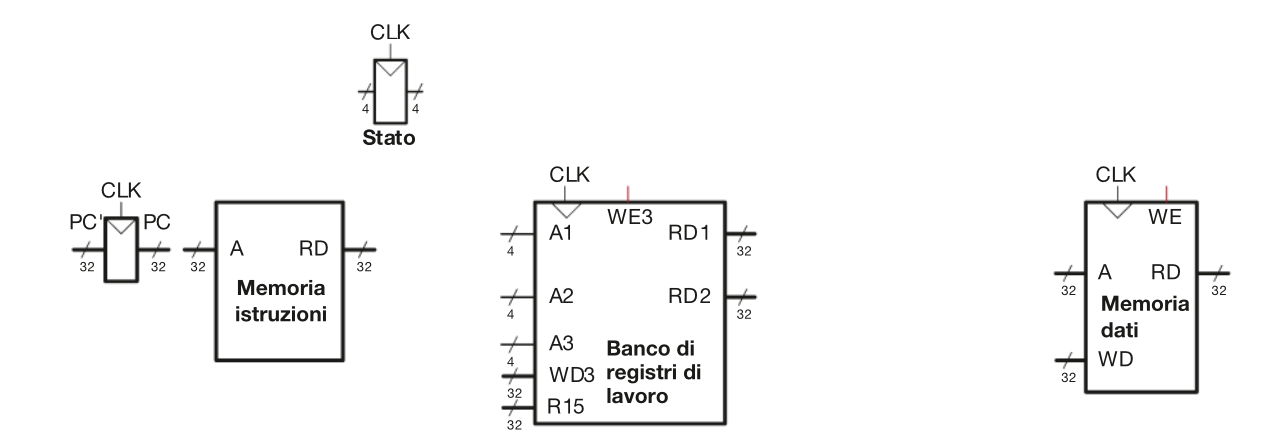
\includegraphics[scale=0.3]{arm_hw.png}
\end{center}
\begin{itemize}
	\item \textbf{Program counter}: concettualmente è parte del banco dei registri, ma dato che viene letto e scritto ad ogni ciclo indipendentemente dall'operazione, conviene realizzarlo separatamente.
	\begin{itemize}
		\item \textit{PC}: istruzione corrente
		\item \textit{PC'}: istruzione successiva
	\end{itemize}
	\item \textbf{Memoria istruzioni}:
	\begin{itemize}
		\item \textit{A}: indirizzo di istruzione a $32$bit
		\item \textit{RD}: l'istruzione
	\end{itemize}
	\item \textbf{Banco di registri}: contiene $15$ elementi da $32$bit
	\begin{itemize}
		\item Due porte di \textbf{lettura} \textit{A1} e \textit{A2} che ricevono indirizzi a $4$ bit per specificare il registro il cui contenuto viene poi emesso su \textit{RD1} e \textit{RD2} a $32$ bit
		\item Una porta di \textbf{scrittura} \textit{A3} che riceve l'indirizzo del registro a $4$ bit e \textit{WD3} che riceve il dato a $32$ bit ed è abilitata da \textit{WE3}
		\item \textbf{R15}, ovvero il \textit{PC}, la quale lettura restituisce $PC + 8$
	\end{itemize}
	\item \textbf{Memoria dati}:
	\begin{itemize}
		\item Singola porta di lettura e scrittura \textit{A}, abilitata da \textit{WE}
		\item \textit{WD}: eventuale dato da scrivere
		\item \textit{RD}: se non c'è l'abilitazione alla scrittura, restituisce il dato della lettura
	\end{itemize}
\end{itemize}
\subsubsection{Tipologie}
Esistono tre tipi di microarchitetture ARM:
\begin{itemize}
	\item \textbf{Ciclo singolo}: esegue una istruzione in un ciclo. Di conseguenza non ha bisogno dello stato architetturale ma il tempo di ciclo è deciso dall'istruzione più lenta
	\item \textbf{Multiciclo}: esegue le istruzioni in sequenze di cicli brevi. Quelle semplici sono eseguite in meno cicli di quelle complesse. Riduce il costo HW riutilizzando componenti come il sommatore
	\item \textbf{Pipeline}: può eseguire più istruzioni contemporaneamente ma necessita di più logica per gestire le dipendenze tra le istruzioni
\end{itemize}

\subsubsection{Prestazioni}
L'analisi consiste nel misurare il tempo di esecuzione di un dato programma su architetture diverse.
\begin{equation}
	t_{esecuzione} = (n_{istruzioni})\bigg(\frac{cicli}{istruzione}\bigg)\bigg(\frac{secondi}{ciclo}\bigg)
\end{equation}
Analizziamo le singole componenti:
\begin{itemize}
	\item \textbf{Numero di istruzioni}: dipende dall'architettura presa in considerazione e dalla bravura del programmatore
	\item \textbf{Cicli per istruzione} (\textbf{CPI}): il numero di cicli di clock richiesti in media per eseguire un'istruzione. È il reciproco della potenza di elaborazione (\textbf{IPC}). Dipende dalla microarchitettura.
	\item \textbf{Secondi per ciclo}, \textbf{$T_c$}: è il periodo del clock. È determinato dal percorso critico attraverso i circuiti del processore. Dipende dal progetto delle reti logiche e dei circuiti (e.g. sommatore ad anticipazione di riporto più veloce di quello a onda di riporto)
\end{itemize}

\subsection{Ciclo singolo}
\begin{center}
	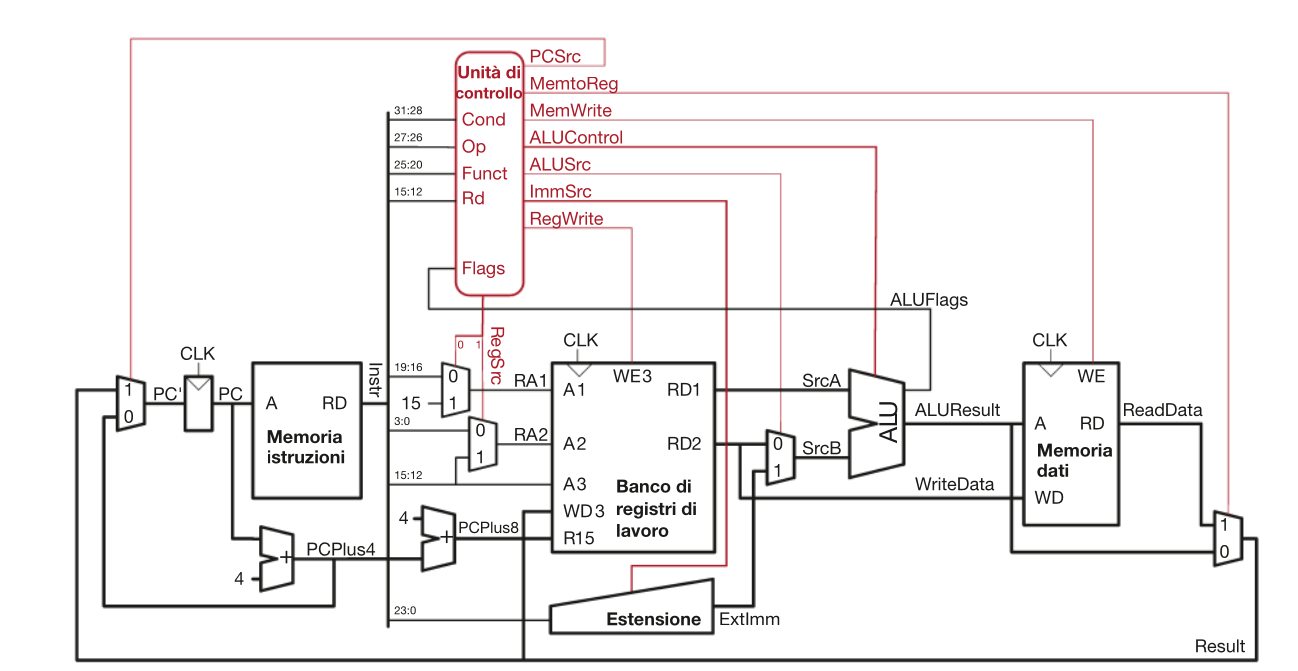
\includegraphics[scale=0.3]{single_cycle.png}
\end{center}
\subsection{Multiciclo}
\subsection{Pipeline}